\section{Introduction}
\label{sec:intro}
Combinatorial search problems are fundamental to computer science and artificial intelligence, with applications in logistics, scheduling, bioinformatics, and puzzle solving. The Futoshiki puzzle, a Japanese constraint satisfaction problem, serves as an excellent benchmark for evaluating algorithmic approaches to these challenges.

Futoshiki requires filling an N×N grid with numbers from 1 to N while satisfying two constraint types: the Latin Square property (each number appears exactly once per row and column) and inequality constraints between adjacent cells. These inequality constraints, represented by $<$ and $>$ symbols, create dependencies that distinguish Futoshiki from standard Latin Square puzzles.

\begin{figure}[H]
\centering
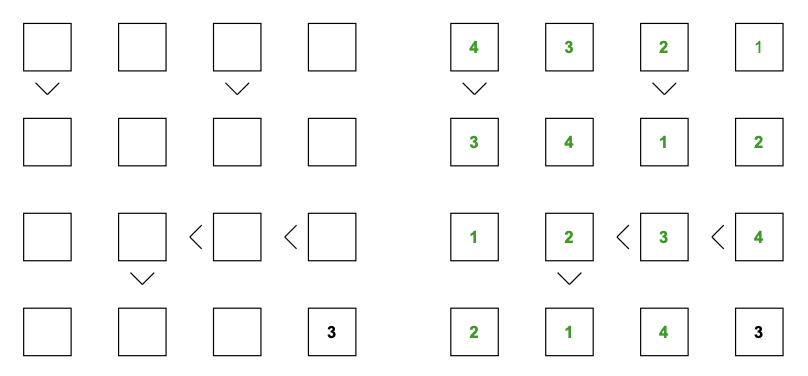
\includegraphics[scale=0.6]{imgs/futoshiki_example.png}
\caption{Example of a Futoshiki puzzle and its solved counterpart \cite{Sen2024Futoshiki}}
\label{fig:futoshiki_example}
\end{figure}

The computational challenge lies not only in Futoshiki's NP-Complete complexity but also in the irregular constraint patterns that make difficulty unpredictable from basic parameters like grid size alone. The arbitrary placement of inequality constraints creates variable search space sizes even for puzzles with identical dimensions and constraint counts.

Recent work by Şen and Diner \cite{Sen2024Futoshiki} demonstrated that transforming Futoshiki into a list coloring problem enables polynomial-time constraint propagation that significantly reduces search space. However, even with these optimizations, challenging puzzles require substantial computational resources, making them suitable targets for parallel computing approaches.

This paper presents a parallel computing framework exploring three paradigms: distributed-memory parallelism using MPI, shared-memory parallelism using OpenMP, and a hybrid approach combining both. Our implementation contributes a dynamic work generation strategy that adapts to puzzle characteristics and available parallelism, along with comprehensive performance analysis across different computational scales.

\subsection{Outline of the paper}
The remainder of this paper is organized as follows. \Cref{sec:related_work} reviews relevant background on constraint satisfaction and parallel puzzle solving. \Cref{sec:solution} describes our sequential baseline implementation and three parallel approaches. \Cref{sec:evaluation} presents experimental methodology and performance analysis across different puzzle characteristics. \Cref{sec:conclusion} and \Cref{sec:future_work} conclude with findings and future research directions.